% Fig. 1 -- accelerator block diagram (TikZ, single column). Structure per v2/docs/ARCH_SPEC.md.
\begin{figure}[t]
\centering
\resizebox{\columnwidth}{!}{%
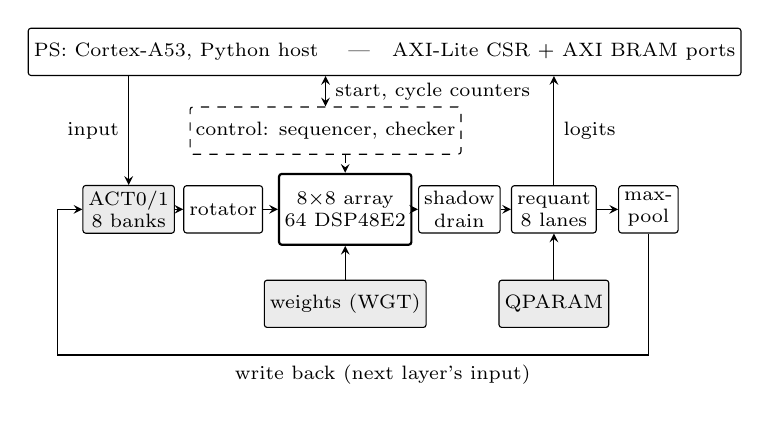
\begin{tikzpicture}[font=\scriptsize, >=stealth,
  blk/.style={draw, rounded corners=1pt, align=center, inner sep=2pt, minimum height=6mm},
  mem/.style={blk, fill=black!8},
  ctl/.style={blk, dashed}]
  % PS
  \node[blk, minimum width=7.9cm] (ps) at (-0.3,2.75)
      {PS: Cortex-A53, Python host \quad|\quad AXI-Lite CSR + AXI BRAM ports};
  % datapath (one row, left to right)
  \node[mem] (act)  at (-3.55,0.75) {ACT0/1\\8 banks};
  \node[blk] (rot)  at (-2.35,0.75) {rotator};
  \node[blk, line width=0.8pt, minimum height=9mm] (arr) at (-0.8,0.75) {$8{\times}8$ array\\64 DSP48E2};
  \node[blk] (drn)  at (0.65,0.75) {shadow\\drain};
  \node[blk] (rq)   at (1.85,0.75) {requant\\8 lanes};
  \node[blk] (pool) at (3.05,0.75) {max-\\pool};
  % memories and control (second row)
  \node[mem] (wgt) at (-0.8,-0.45) {weights (WGT)};
  \node[mem] (qp)  at (1.85,-0.45) {QPARAM};
  \node[ctl] (seq) at (-1.05,1.75) {control: sequencer, checker};
  % data flow
  \draw[->] (act) -- (rot);
  \draw[->] (rot) -- (arr);
  \draw[->] (arr) -- (drn);
  \draw[->] (drn) -- (rq);
  \draw[->] (rq) -- (pool);
  \draw[->] (wgt) -- (arr);
  \draw[->] (qp) -- (rq);
  \draw[->] (pool.south) -- (3.05,-1.1) -- (-4.45,-1.1) node[pos=0.45, below] {write back (next layer's input)} -- (-4.45,0.75) -- (act.west);
  \draw[dashed,->] (seq.south -| arr.north) -- (arr.north);
  % host interface
  \draw[->] (act.north |- ps.south) -- (act.north) node[pos=0.5, left] {input};
  \draw[<->] (seq.north |- ps.south) -- (seq.north) node[midway, right] {start, cycle counters};
  \draw[->] (rq.north) -- (rq.north |- ps.south) node[midway, right] {logits};
\end{tikzpicture}}
\caption{Accelerator organization. Weights and activations stay in BRAM; the host writes the input,
starts a job and reads the logits and cycle counters.}
\label{fig:arch}
\end{figure}
